\chapter{Impact Analysis}\newpage

\section{Introduction}

The model evaluation distinguishes three fiscal aggregates used for policy interpretation: 

\begin{itemize}
    \item \textbf{Total Actual Cost} --- the sum of all observed expenditures in the historical dataset for the base year.  This represents the agency's actual fiscal outlay for waiver services and serves as the empirical baseline.  
    \item \textbf{Total Predicted Cost} --- the sum of the model's estimated allocations for each individual, based solely on assessed need and model parameters.  This reflects the theoretical distribution of funds if the predictive algorithm were implemented without any legal or policy constraints.  
    \item \textbf{Total Compliant Budget} --- this measure enforces statutory protections against reductions in individual allocations by setting each person's projected cost to the greater of the actual and predicted values, that is, 
    $\text{Compliant}_i = \max(\text{Actual}_i, \text{Predicted}_i)$.  
    The Total Compliant Budget therefore guarantees that no participant receives less than their current level of support, ensuring compliance with legislative requirements such as F.S.~393.0662.  
\end{itemize}

% Economic Impact Analysis Report
% Generated: 2025-10-13 17:57:32
% Conservative Budget Estimation Analysis

\section{Economic Impact Analysis}
\label{sec:economic_impact}

This section presents the economic impact analysis for each budget allocation model. The conservative budget estimate is defined as the maximum of the actual cost and predicted cost for each case: $\text{Conservative} = \max(\text{Actual}, \text{Predicted})$. This approach ensures adequate funding while accounting for model uncertainty.

\subsection{Model 1: Impact Analysis}
\label{subsec:model1_impact}

\begin{table}[htbp]
\centering
\small
\caption{Model 1: Economic Impact Summary}
\label{tab:model1_impact_summary}
\begin{tabular}{lrr}
\toprule
\textbf{Metric} & \textbf{Value} & \textbf{Per Client} \\
\midrule
Sample Size & 6,834 & --- \\
\midrule
Total Actual Cost & \$302,173,388.29 & \$44,216.18 \\
Total Predicted Cost & \$254,727,261.09 & \$37,273.52 \\
Total Conservative Budget & \$352,936,104.68 & \$51,644.15 \\
\midrule
\textbf{Economic Impact} & \textbf{\$+50,762,716.39} & \textbf{\$+7,427.97} \\
Impact Percentage & 16.80\% & --- \\
\midrule
Cases Over Budget & 3,547 & 51.9\% \\
\midrule
Model $R^2$ (Test) & 0.4300 & --- \\
RMSE (Test) & \$33,718.68 & --- \\
\bottomrule
\end{tabular}
\end{table}

Figure~\ref{fig:model1_impact_histograms} presents the distribution analysis for Model 1, showing the distributions of actual costs, predicted costs, prediction errors, and conservative budget estimates.

\begin{figure}[htbp]
\centering
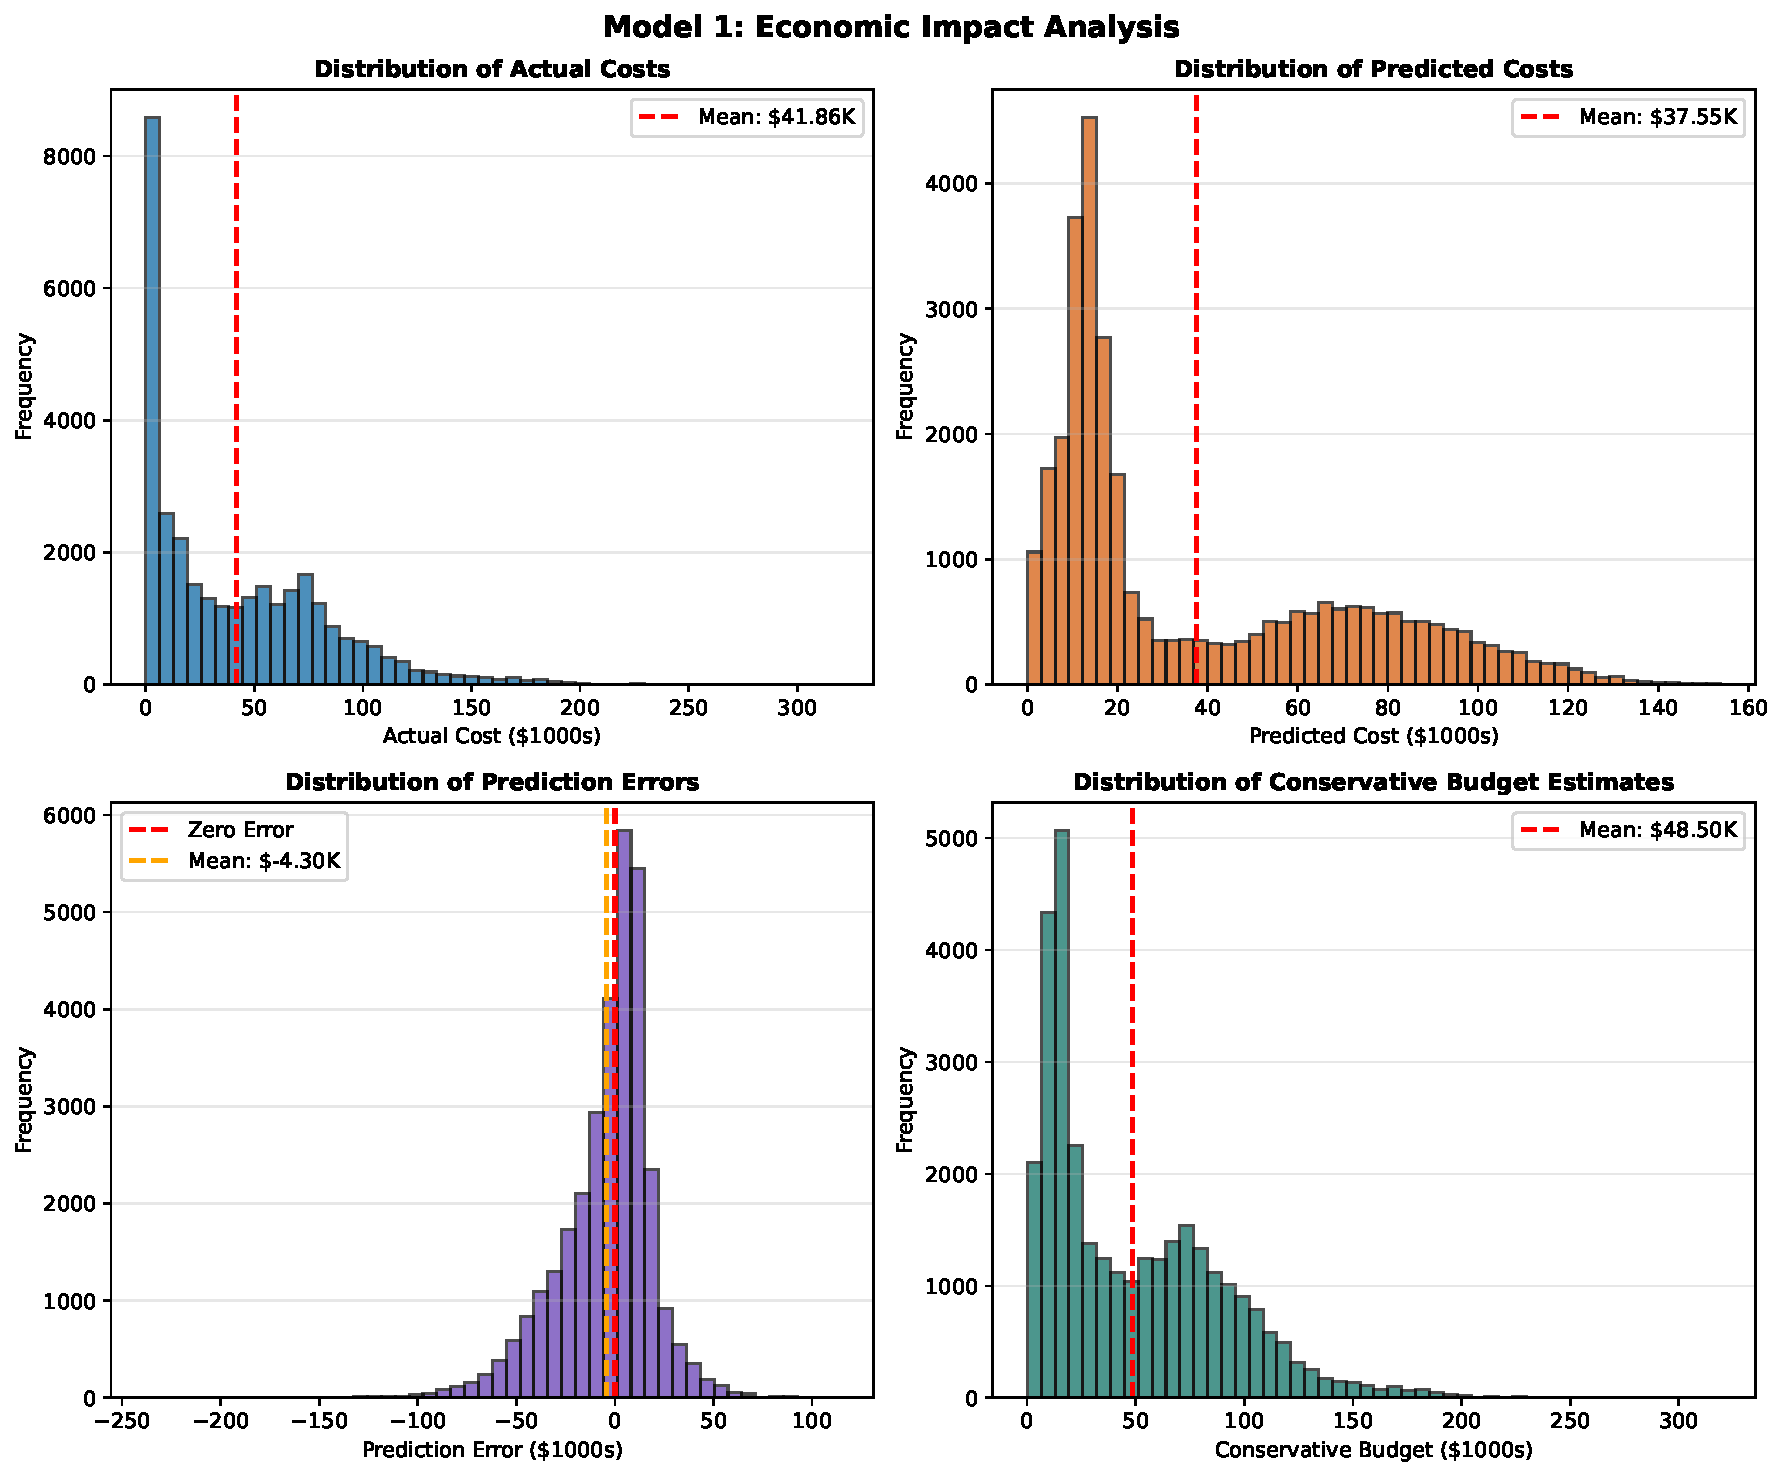
\includegraphics[width=0.95\textwidth]{figures/model_1_Impact_Histograms.pdf}
\caption{Model 1: Distribution of costs, predictions, errors, and conservative budget estimates. The conservative estimate takes the maximum of actual and predicted costs to ensure adequate funding.}
\label{fig:model1_impact_histograms}
\end{figure}

The conservative budgeting approach for Model 1 would require an additional \$50,762,716.39 (16.80\%) compared to actual costs, averaging \$7,427.97 per client. The model under-predicted costs in 51.9\% of cases, necessitating the conservative approach to avoid budget shortfalls.

\clearpage

\subsection{Model 2: Impact Analysis}
\label{subsec:model2_impact}

\begin{table}[htbp]
\centering
\small
\caption{Model 2: Economic Impact Summary}
\label{tab:model2_impact_summary}
\begin{tabular}{lrr}
\toprule
\textbf{Metric} & \textbf{Value} & \textbf{Per Client} \\
\midrule
Sample Size & 6,834 & --- \\
\midrule
Total Actual Cost & \$302,173,388.29 & \$44,216.18 \\
Total Predicted Cost & \$280,247,265.15 & \$41,007.79 \\
Total Conservative Budget & \$368,832,113.67 & \$53,970.17 \\
\midrule
\textbf{Economic Impact} & \textbf{\$+66,658,725.38} & \textbf{\$+9,753.98} \\
Impact Percentage & 22.06\% & --- \\
\midrule
Cases Over Budget & 3,909 & 57.2\% \\
\midrule
Model $R^2$ (Test) & 0.4252 & --- \\
RMSE (Test) & \$33,859.02 & --- \\
\bottomrule
\end{tabular}
\end{table}

Figure~\ref{fig:model2_impact_histograms} presents the distribution analysis for Model 2, showing the distributions of actual costs, predicted costs, prediction errors, and conservative budget estimates.

\begin{figure}[htbp]
\centering
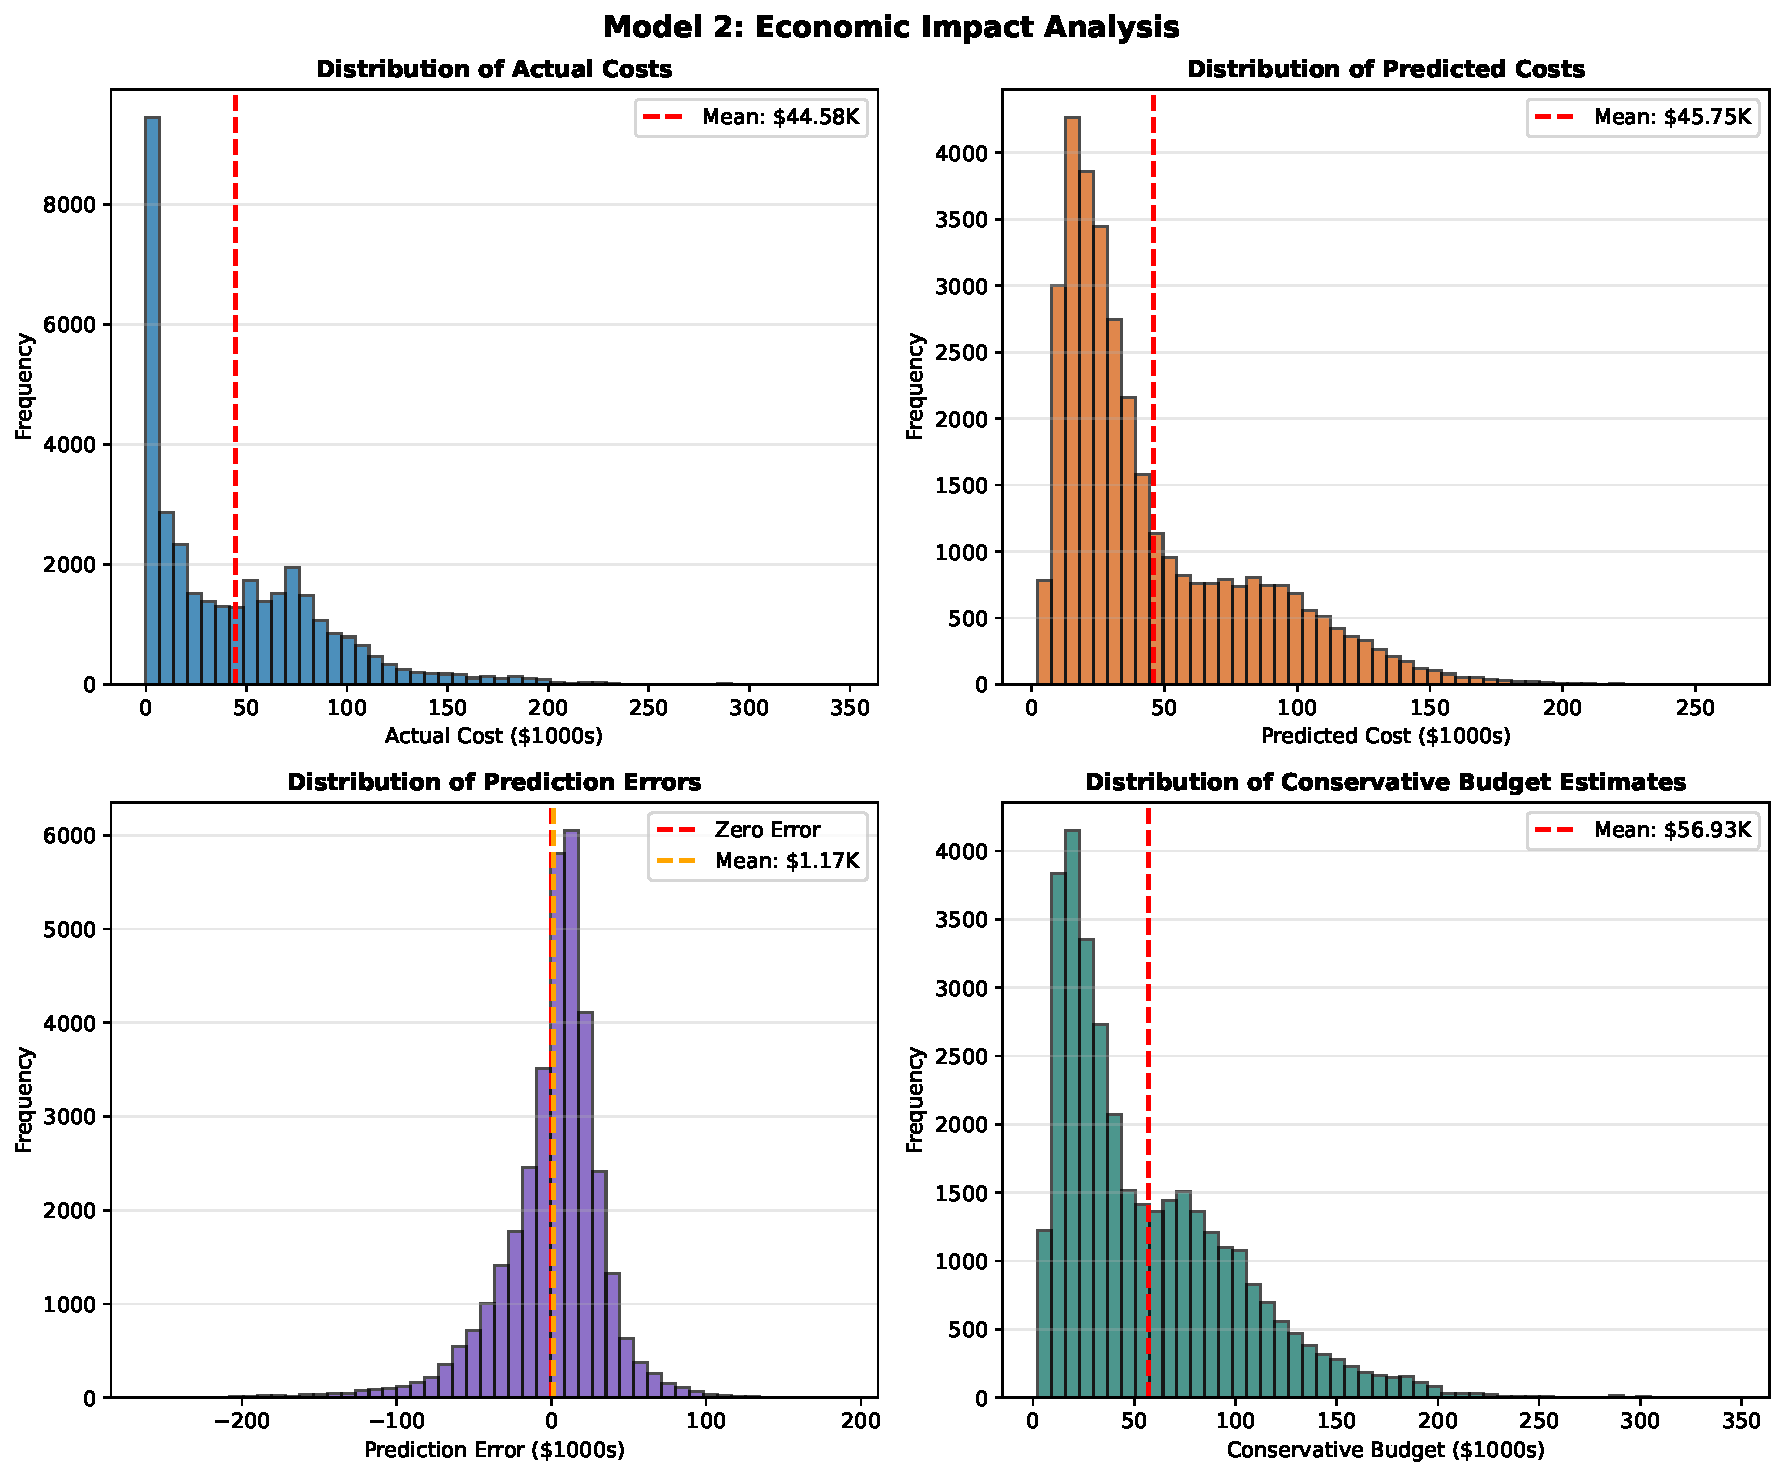
\includegraphics[width=0.95\textwidth]{figures/model_2_Impact_Histograms.pdf}
\caption{Model 2: Distribution of costs, predictions, errors, and conservative budget estimates. The conservative estimate takes the maximum of actual and predicted costs to ensure adequate funding.}
\label{fig:model2_impact_histograms}
\end{figure}

The conservative budgeting approach for Model 2 would require an additional \$66,658,725.38 (22.06\%) compared to actual costs, averaging \$9,753.98 per client. The model under-predicted costs in 57.2\% of cases, necessitating the conservative approach to avoid budget shortfalls.

\clearpage

\subsection{Model 3: Impact Analysis}
\label{subsec:model3_impact}

\begin{table}[htbp]
\centering
\small
\caption{Model 3: Economic Impact Summary}
\label{tab:model3_impact_summary}
\begin{tabular}{lrr}
\toprule
\textbf{Metric} & \textbf{Value} & \textbf{Per Client} \\
\midrule
Sample Size & 6,834 & --- \\
\midrule
Total Actual Cost & \$302,173,388.29 & \$44,216.18 \\
Total Predicted Cost & \$253,500,237.16 & \$37,093.98 \\
Total Conservative Budget & \$352,264,517.13 & \$51,545.88 \\
\midrule
\textbf{Economic Impact} & \textbf{\$+50,091,128.84} & \textbf{\$+7,329.69} \\
Impact Percentage & 16.58\% & --- \\
\midrule
Cases Over Budget & 3,508 & 51.3\% \\
\midrule
Model $R^2$ (Test) & 0.4317 & --- \\
RMSE (Test) & \$33,666.51 & --- \\
\bottomrule
\end{tabular}
\end{table}

Figure~\ref{fig:model3_impact_histograms} presents the distribution analysis for Model 3, showing the distributions of actual costs, predicted costs, prediction errors, and conservative budget estimates.

\begin{figure}[htbp]
\centering
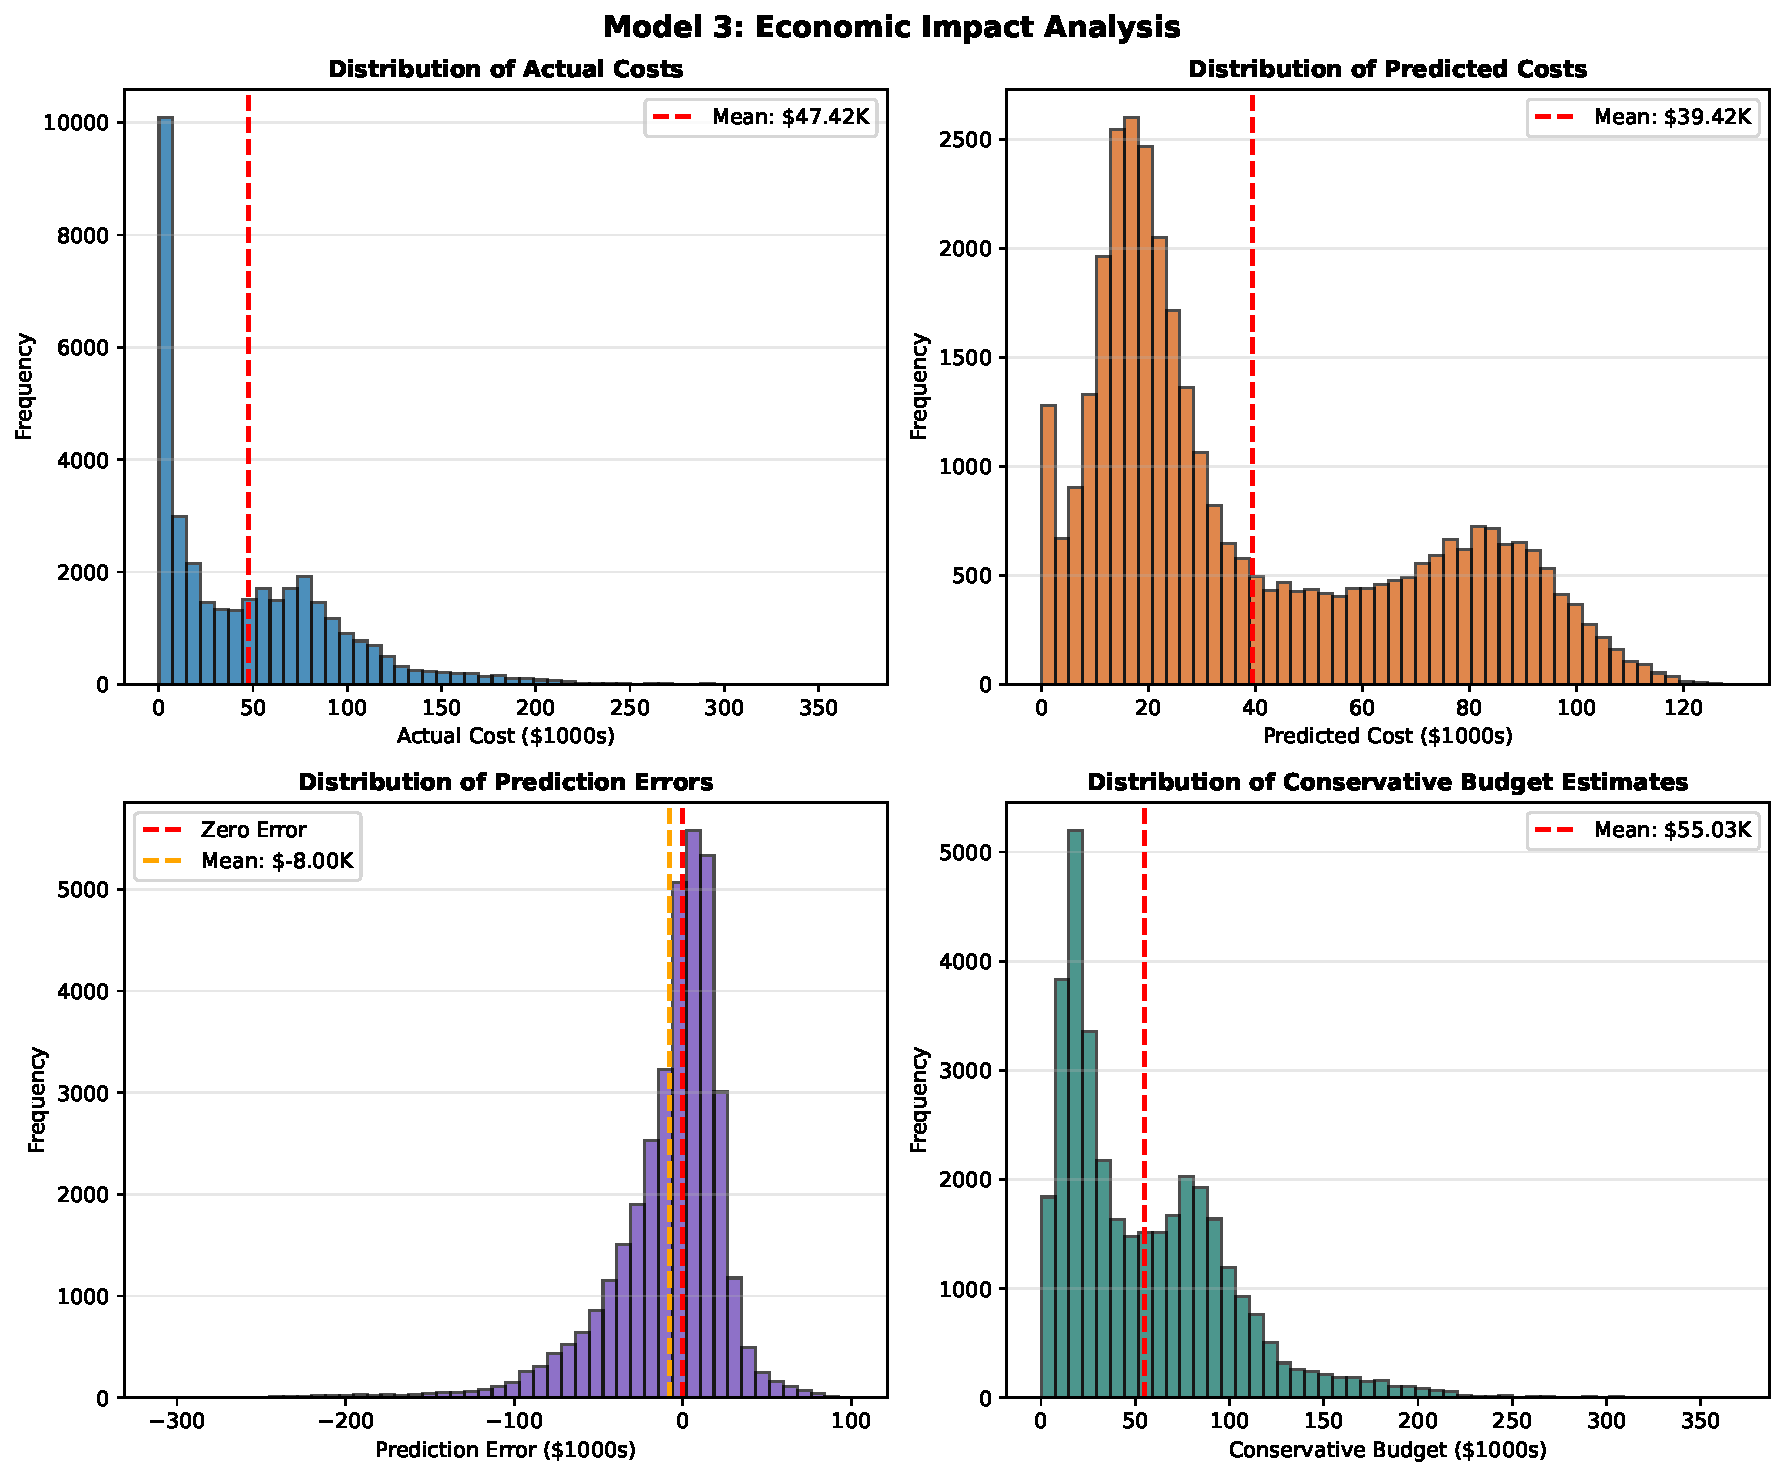
\includegraphics[width=0.95\textwidth]{figures/model_3_Impact_Histograms.pdf}
\caption{Model 3: Distribution of costs, predictions, errors, and conservative budget estimates. The conservative estimate takes the maximum of actual and predicted costs to ensure adequate funding.}
\label{fig:model3_impact_histograms}
\end{figure}

The conservative budgeting approach for Model 3 would require an additional \$50,091,128.84 (16.58\%) compared to actual costs, averaging \$7,329.69 per client. The model under-predicted costs in 51.3\% of cases, necessitating the conservative approach to avoid budget shortfalls.

\clearpage

\subsection{Model 4: Impact Analysis}
\label{subsec:model4_impact}

\begin{table}[htbp]
\centering
\small
\caption{Model 4: Economic Impact Summary}
\label{tab:model4_impact_summary}
\begin{tabular}{lrr}
\toprule
\textbf{Metric} & \textbf{Value} & \textbf{Per Client} \\
\midrule
Sample Size & 6,834 & --- \\
\midrule
Total Actual Cost & \$302,173,388.29 & \$44,216.18 \\
Total Predicted Cost & \$301,205,398.71 & \$44,074.54 \\
Total Conservative Budget & \$378,953,638.78 & \$55,451.22 \\
\midrule
\textbf{Economic Impact} & \textbf{\$+76,780,250.49} & \textbf{\$+11,235.04} \\
Impact Percentage & 25.41\% & --- \\
\midrule
Cases Over Budget & 4,042 & 59.1\% \\
\midrule
Model $R^2$ (Test) & 0.4717 & --- \\
RMSE (Test) & \$32,462.66 & --- \\
\bottomrule
\end{tabular}
\end{table}

Figure~\ref{fig:model4_impact_histograms} presents the distribution analysis for Model 4, showing the distributions of actual costs, predicted costs, prediction errors, and conservative budget estimates.

\begin{figure}[htbp]
\centering
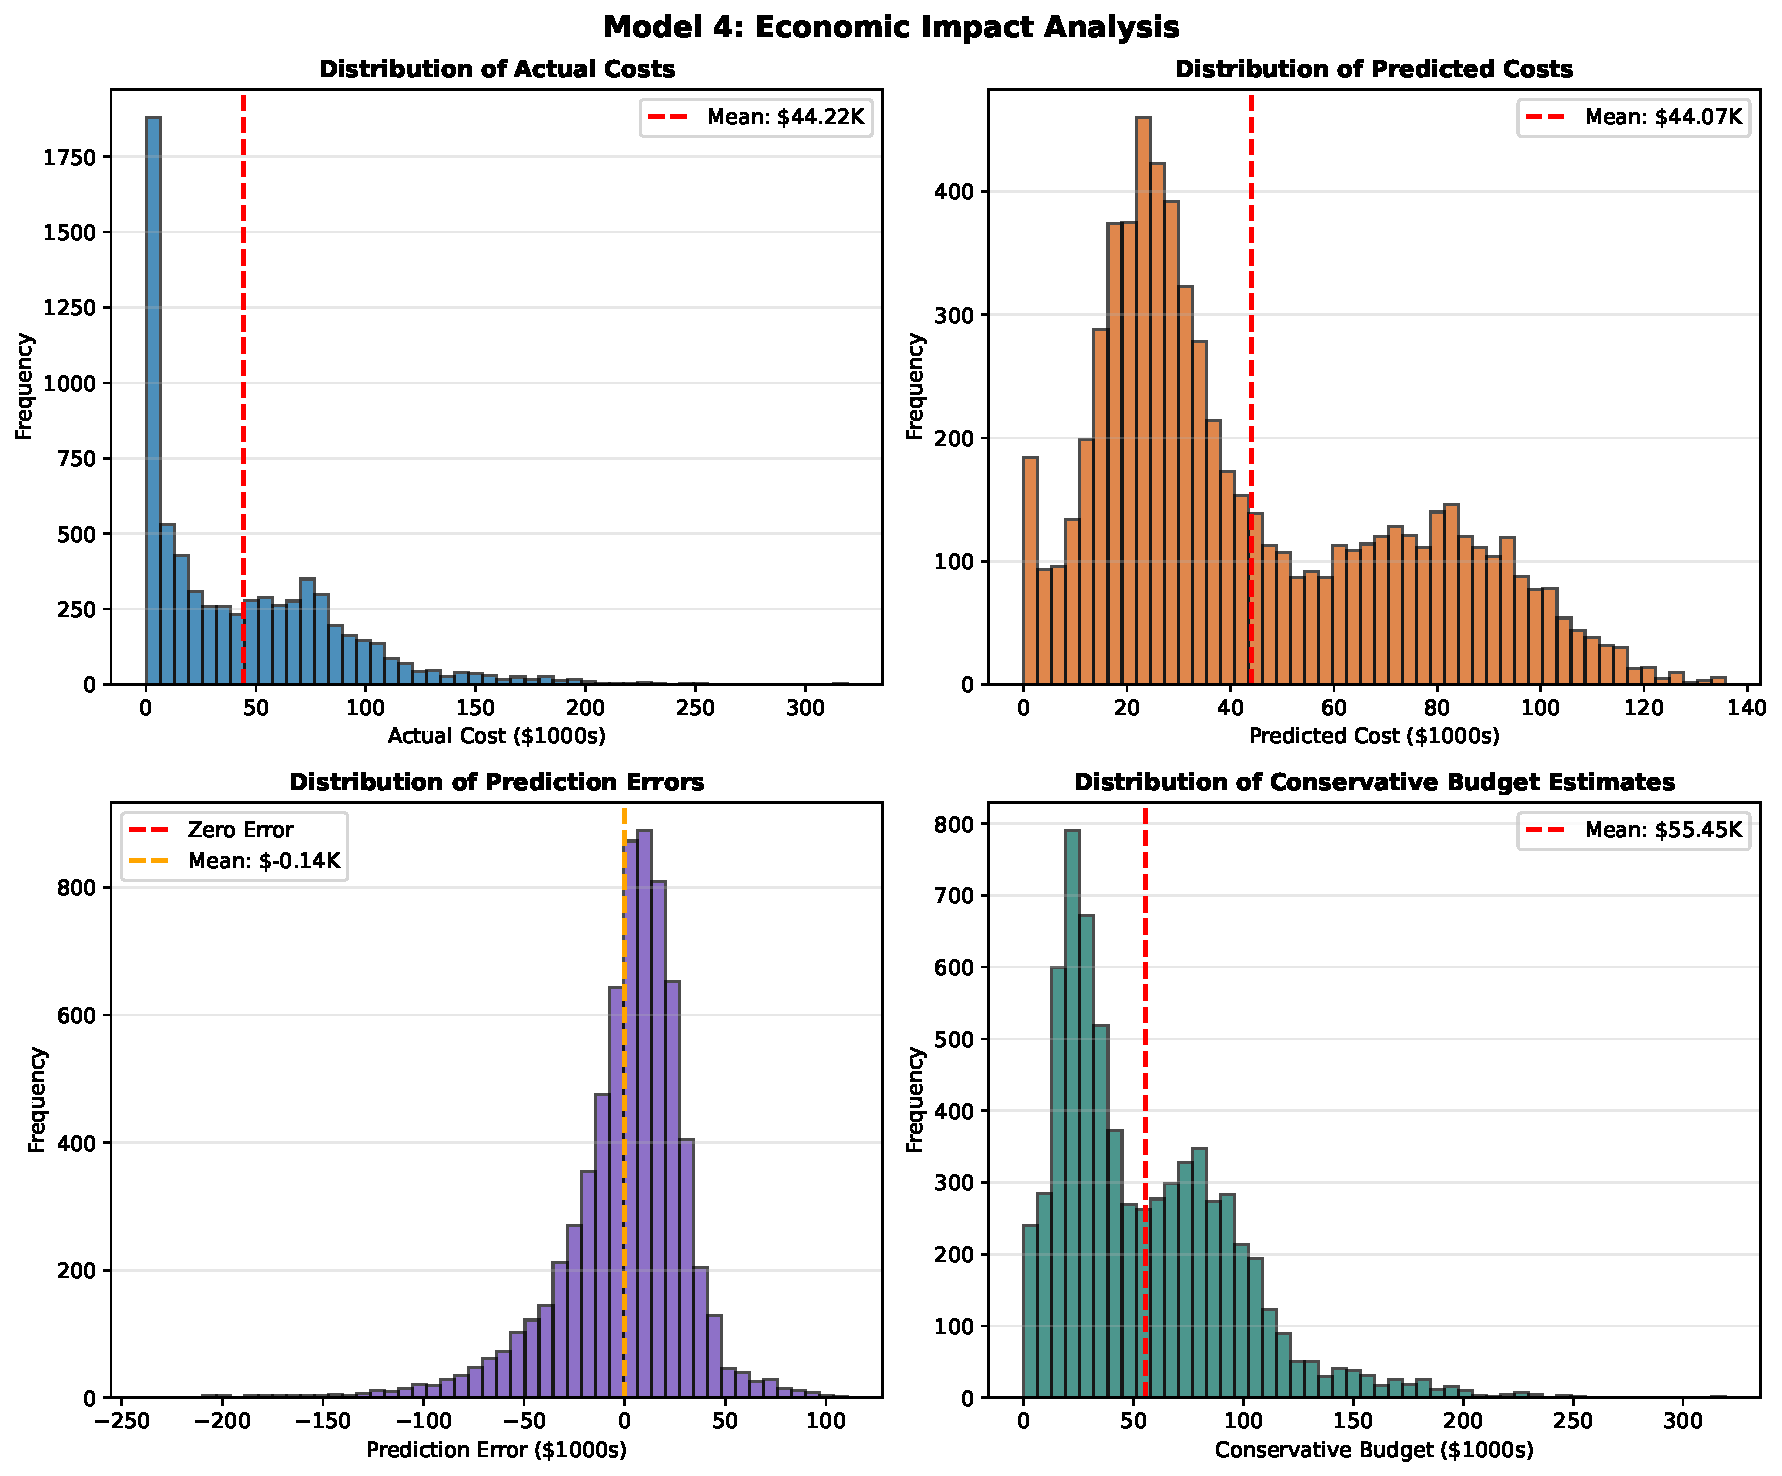
\includegraphics[width=0.95\textwidth]{figures/model_4_Impact_Histograms.pdf}
\caption{Model 4: Distribution of costs, predictions, errors, and conservative budget estimates. The conservative estimate takes the maximum of actual and predicted costs to ensure adequate funding.}
\label{fig:model4_impact_histograms}
\end{figure}

The conservative budgeting approach for Model 4 would require an additional \$76,780,250.49 (25.41\%) compared to actual costs, averaging \$11,235.04 per client. The model under-predicted costs in 59.1\% of cases, necessitating the conservative approach to avoid budget shortfalls.

\clearpage

\subsection{Model 5: Impact Analysis}
\label{subsec:model5_impact}

\begin{table}[htbp]
\centering
\small
\caption{Model 5: Economic Impact Summary}
\label{tab:model5_impact_summary}
\begin{tabular}{lrr}
\toprule
\textbf{Metric} & \textbf{Value} & \textbf{Per Client} \\
\midrule
Sample Size & 6,834 & --- \\
\midrule
Total Actual Cost & \$302,173,388.29 & \$44,216.18 \\
Total Predicted Cost & \$260,331,382.59 & \$38,093.56 \\
Total Conservative Budget & \$356,096,831.54 & \$52,106.65 \\
\midrule
\textbf{Economic Impact} & \textbf{\$+53,923,443.25} & \textbf{\$+7,890.47} \\
Impact Percentage & 17.85\% & --- \\
\midrule
Cases Over Budget & 3,576 & 52.3\% \\
\midrule
Model $R^2$ (Test) & 0.4474 & --- \\
RMSE (Test) & \$33,198.10 & --- \\
\bottomrule
\end{tabular}
\end{table}

Figure~\ref{fig:model5_impact_histograms} presents the distribution analysis for Model 5, showing the distributions of actual costs, predicted costs, prediction errors, and conservative budget estimates.

\begin{figure}[htbp]
\centering
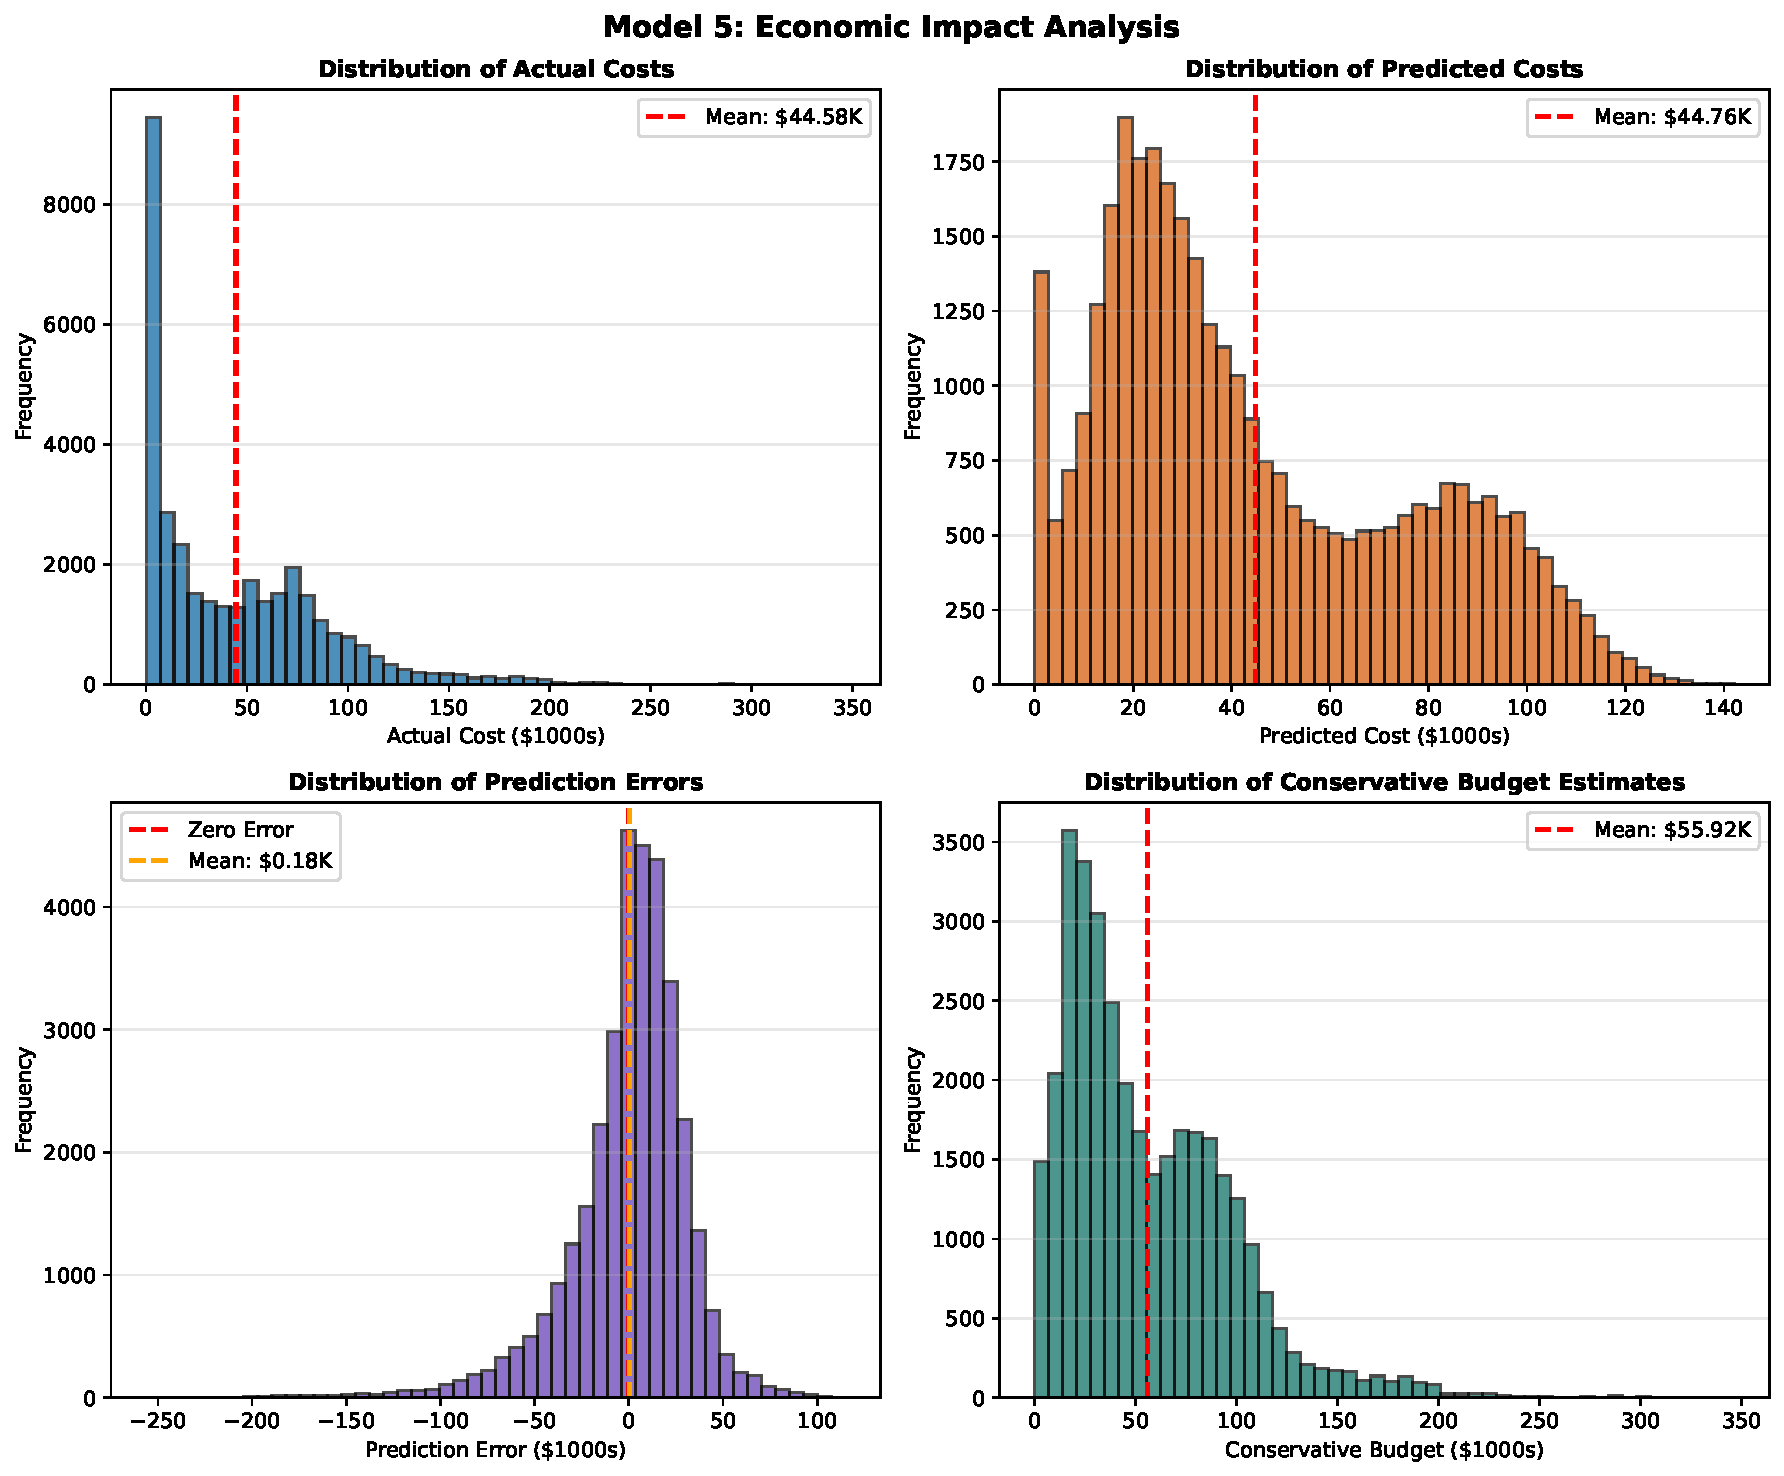
\includegraphics[width=0.95\textwidth]{figures/model_5_Impact_Histograms.pdf}
\caption{Model 5: Distribution of costs, predictions, errors, and conservative budget estimates. The conservative estimate takes the maximum of actual and predicted costs to ensure adequate funding.}
\label{fig:model5_impact_histograms}
\end{figure}

The conservative budgeting approach for Model 5 would require an additional \$53,923,443.25 (17.85\%) compared to actual costs, averaging \$7,890.47 per client. The model under-predicted costs in 52.3\% of cases, necessitating the conservative approach to avoid budget shortfalls.

\clearpage

\subsection{Model 6: Impact Analysis}
\label{subsec:model6_impact}

\begin{table}[htbp]
\centering
\small
\caption{Model 6: Economic Impact Summary}
\label{tab:model6_impact_summary}
\begin{tabular}{lrr}
\toprule
\textbf{Metric} & \textbf{Value} & \textbf{Per Client} \\
\midrule
Sample Size & 6,834 & --- \\
\midrule
Total Actual Cost & \$302,173,388.29 & \$44,216.18 \\
Total Predicted Cost & \$413,605,889.79 & \$60,521.79 \\
Total Conservative Budget & \$477,292,383.97 & \$69,840.85 \\
\midrule
\textbf{Economic Impact} & \textbf{\$+175,118,995.68} & \textbf{\$+25,624.67} \\
Impact Percentage & 57.95\% & --- \\
\midrule
Cases Over Budget & 4,818 & 70.5\% \\
\midrule
Model $R^2$ (Test) & -0.3008 & --- \\
RMSE (Test) & \$50,935.97 & --- \\
\bottomrule
\end{tabular}
\end{table}

Figure~\ref{fig:model6_impact_histograms} presents the distribution analysis for Model 6, showing the distributions of actual costs, predicted costs, prediction errors, and conservative budget estimates.

\begin{figure}[htbp]
\centering
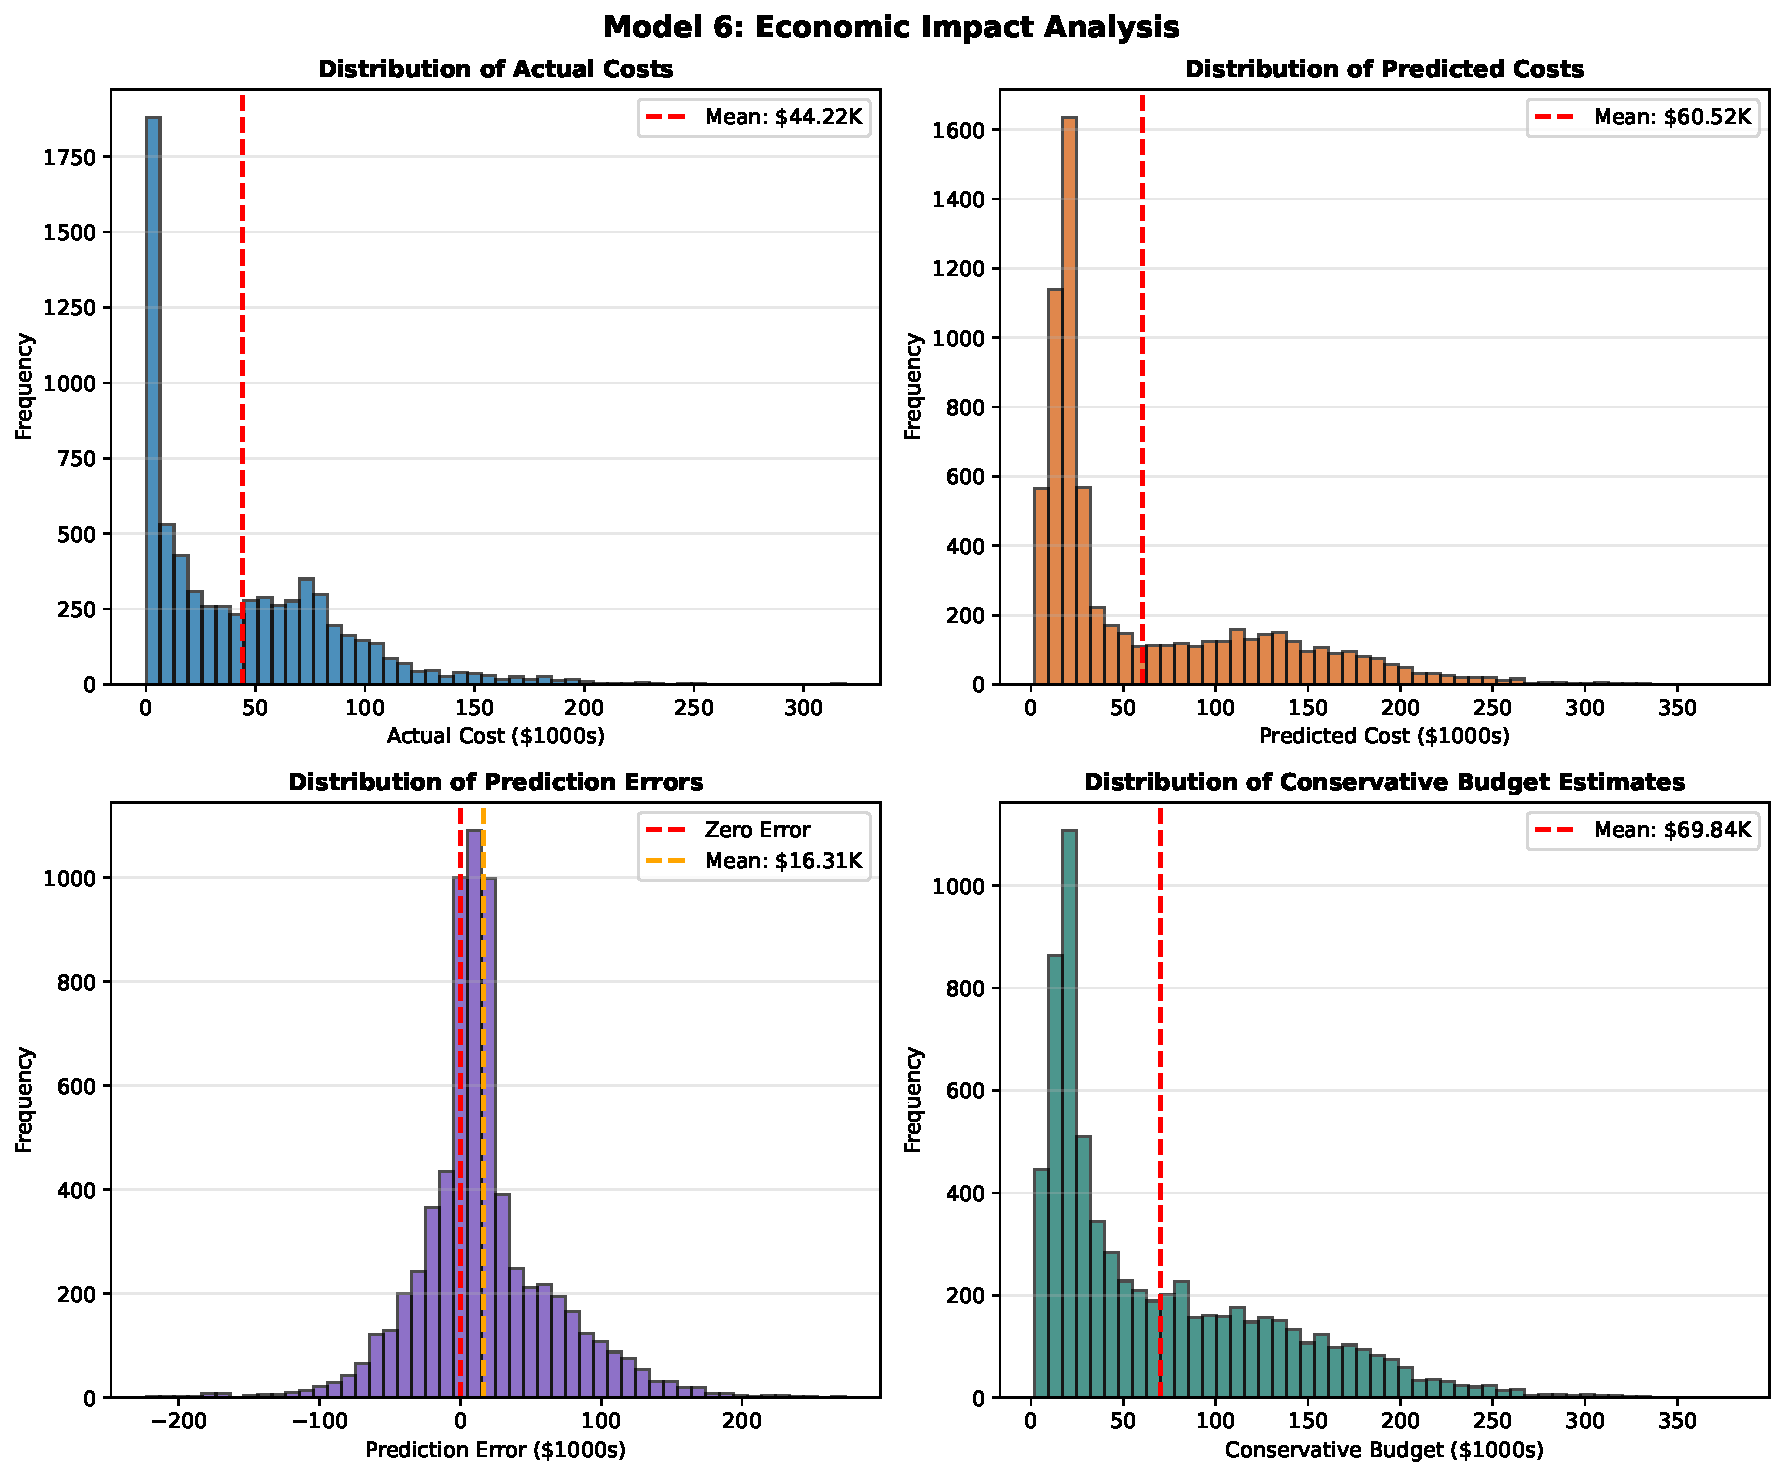
\includegraphics[width=0.95\textwidth]{figures/model_6_Impact_Histograms.pdf}
\caption{Model 6: Distribution of costs, predictions, errors, and conservative budget estimates. The conservative estimate takes the maximum of actual and predicted costs to ensure adequate funding.}
\label{fig:model6_impact_histograms}
\end{figure}

The conservative budgeting approach for Model 6 would require an additional \$175,118,995.68 (57.95\%) compared to actual costs, averaging \$25,624.67 per client. The model under-predicted costs in 70.5\% of cases, necessitating the conservative approach to avoid budget shortfalls.

\clearpage

\subsection{Model 9: Impact Analysis}
\label{subsec:model9_impact}

\begin{table}[htbp]
\centering
\small
\caption{Model 9: Economic Impact Summary}
\label{tab:model9_impact_summary}
\begin{tabular}{lrr}
\toprule
\textbf{Metric} & \textbf{Value} & \textbf{Per Client} \\
\midrule
Sample Size & 19,893 & --- \\
\midrule
Total Actual Cost & \$787,621,455.30 & \$39,592.89 \\
Total Predicted Cost & \$679,742,324.93 & \$34,169.93 \\
Total Conservative Budget & \$915,710,129.65 & \$46,031.78 \\
\midrule
\textbf{Economic Impact} & \textbf{\$+128,088,674.35} & \textbf{\$+6,438.88} \\
Impact Percentage & 16.26\% & --- \\
\midrule
Cases Over Budget & 10,164 & 51.1\% \\
\midrule
Model $R^2$ (Test) & 0.5472 & --- \\
RMSE (Test) & \$27,777.18 & --- \\
\bottomrule
\end{tabular}
\end{table}

Figure~\ref{fig:model9_impact_histograms} presents the distribution analysis for Model 9, showing the distributions of actual costs, predicted costs, prediction errors, and conservative budget estimates.

\begin{figure}[htbp]
\centering
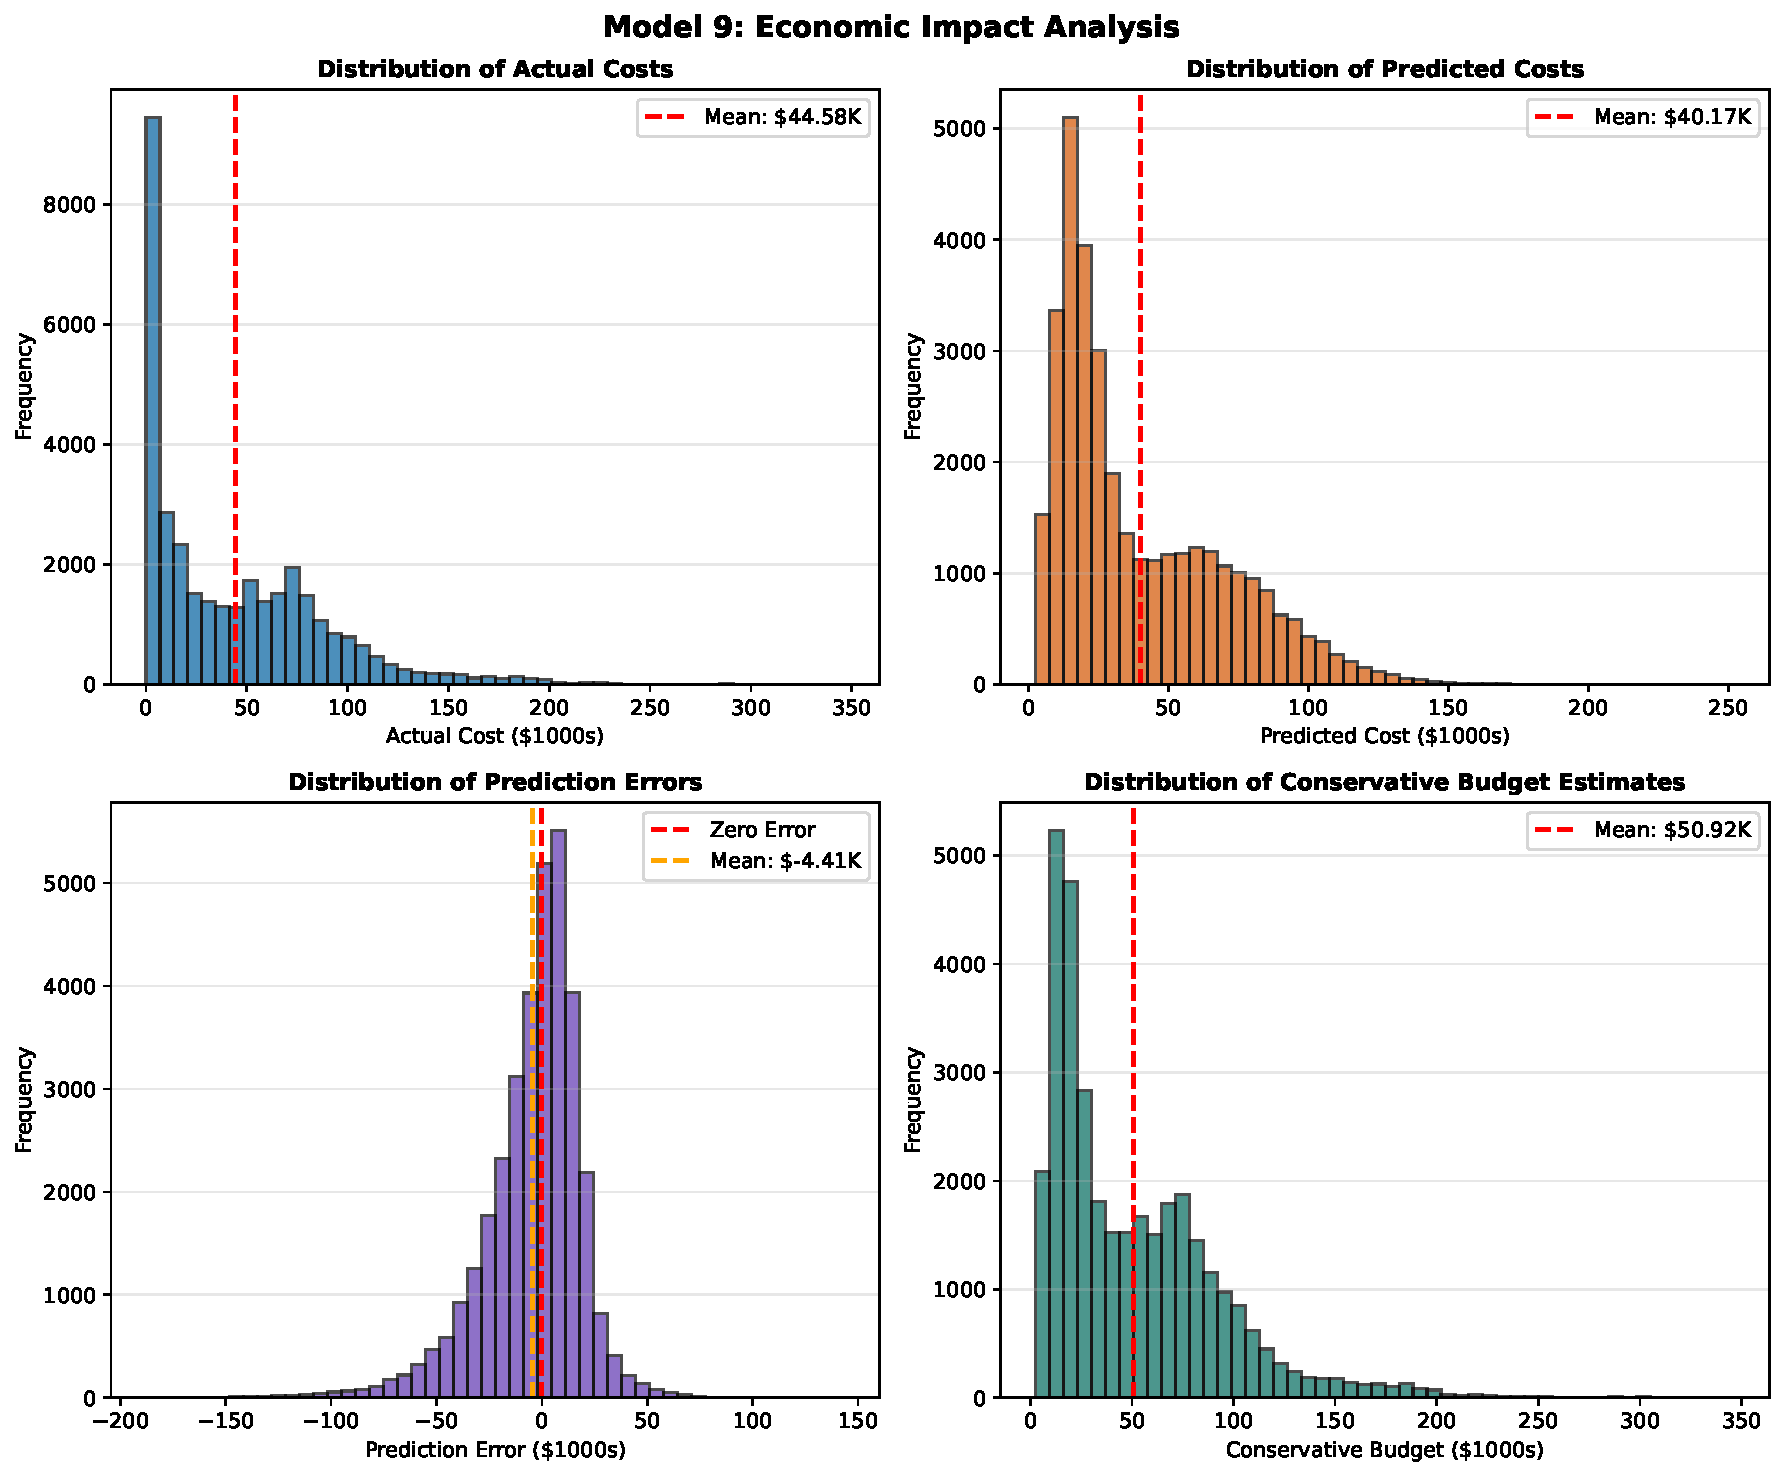
\includegraphics[width=0.95\textwidth]{figures/model_9_Impact_Histograms.pdf}
\caption{Model 9: Distribution of costs, predictions, errors, and conservative budget estimates. The conservative estimate takes the maximum of actual and predicted costs to ensure adequate funding.}
\label{fig:model9_impact_histograms}
\end{figure}

The conservative budgeting approach for Model 9 would require an additional \$128,088,674.35 (16.26\%) compared to actual costs, averaging \$6,438.88 per client. The model under-predicted costs in 51.1\% of cases, necessitating the conservative approach to avoid budget shortfalls.

\clearpage

\subsection{Comparative Analysis Across Models}
\label{subsec:comparative_impact}

Table~\ref{tab:all_models_impact_comparison} presents a comprehensive comparison of economic impacts across all budget allocation models.

\begin{table}[htbp]
\centering
\small
\caption{Comparative Economic Impact Analysis Across All Models}
\label{tab:all_models_impact_comparison}
\begin{tabular}{lrrrrr}
\toprule
\textbf{Model} & \textbf{Samples} & \textbf{$R^2$ Test} & \textbf{Economic Impact} & \textbf{Impact \%} & \textbf{Over Budget \%} \\
\midrule
Model 1 & 6,834 & 0.4300 & \$+50,762,716.39 & +16.80\% & 51.9\% \\
Model 2 & 6,834 & 0.4252 & \$+66,658,725.38 & +22.06\% & 57.2\% \\
Model 3 & 6,834 & 0.4317 & \$+50,091,128.84 & +16.58\% & 51.3\% \\
Model 4 & 6,834 & 0.4717 & \$+76,780,250.49 & +25.41\% & 59.1\% \\
Model 5 & 6,834 & 0.4474 & \$+53,923,443.25 & +17.85\% & 52.3\% \\
Model 6 & 6,834 & -0.3008 & \$+175,118,995.68 & +57.95\% & 70.5\% \\
Model 9 & 19,893 & 0.5472 & \$+128,088,674.35 & +16.26\% & 51.1\% \\
\bottomrule
\end{tabular}
\end{table}

\subsubsection{Key Insights}

\begin{itemize}
\item Model 9 achieves the highest predictive accuracy with $R^2$ = 0.5472.
\item Model 6 requires the largest conservative budget adjustment at 57.95\%.
\item The conservative budgeting approach ensures adequate funding to cover cases where the model under-predicts actual costs.
\item Economic impact percentages reflect both model accuracy and the degree of systematic under- or over-prediction.
\end{itemize}

 